%!TEX root = ../../common/main.tex

\chapter{Tests}

% ---------------------------------------
% Fonts
% ---------------------------------------
\section{Fonts}

\subsection{Blindtext}
\blindtext[3]
\blindlist{itemize}[3]
\blindmathtrue
\blindtext
\blindlist{enumerate}[3]
\blindmathpaper

% ---------------------------------------
% todonotes
% ---------------------------------------
\section{To-do notes}

\blindtext
\info{This is a very informative note}
\blindtext
\todo{A standard to-do note}
\blindtext
\addref{Cite this, cite that}
\blindtext
\missing{Add section about interesting study}
\blindtext
\important{Very urgent stuff!}
The quick brown fox jumps over the lazy dog. Jackdaws love my big
\replace{Jinx}{Sphinx} of Quartz. Pack my box with five dozen liquor jugs.
\blindtext
\redo{Recreate this ugly looking plot and make it nice!}

% ---------------------------------------
% Feynman Diagrams
% ---------------------------------------

\section{Feynman Diagrams}

\begin{tikzpicture}[line width=1.5 pt, scale=1.3]
  \everymath{\displaystyle}
%
  \node[draw,circle] (id1) at (0,1.7em) {$d$};
  \node[draw,circle] (id2) at (0,0em) {$u$};
  \node[draw,circle] (iu1) at (0,-1.7em) {$d$};
%
  \draw[dashed, black!30] (0,0) ellipse (1.8em and 3em);  
%
  \node[draw,circle] (od1) at (8em,1.7em) {$d$};
  \node[draw,circle] (ou1) at (8em,0em) {$u$};
  \node[draw,circle] (ou2) at (8em,-1.7em) {$u$};
%
  \draw[dashed, black!30] (8em,0) ellipse (1.8em and 3em);
%   
  \draw[fermion] (id1) -- (od1);
  \draw[fermion] (id2) -- (ou1);
  \draw[fermion] (iu1) -- (3em,-1.7em);
  \draw[fermion] (3em,-1.7em) -- (ou2);
    \draw[snake=snake, line before snake=.5em] (3em,-1.7em) -- (5em, -4.5em); 
  \draw[fermion] (5em, -4.5em) -- (8em, -4em);
  \draw[fermionbar] (5em, -4.5em) -- (8em, -5.5em);
  % NOTE: snake = snake is important
  \node at (3em,-4em) {$W^+$};
  \node at (8.6em,-4em) {$\nu_e$};
  \node at (8.5em,-5.5em) {$e$};
\end{tikzpicture}


\vspace{1em}

\begin{center}
  \begin{tikzpicture}[line width=1.5 pt, scale=1.3]
    \draw[fermion] (15:1.5)--(0,0);
    \draw[fermionbar] (180:1)--(0,0);
    \draw[vector] (-40:1)--(0,0);
    \node at (15:1.7) {$c$};
    \node at (180:1.2) {$b$};
    \node at (0.75,-.2) {$\Wp$};
    \coordinate (uin) at (-1,-.3);
    \coordinate (umid) at (-80:.5);
  % \begin{scope}[shift={(0,.3)}]
  %   \draw[fermion] (180:1) to [out=0,in=220] (40:1); 
  %   \node at (40:1.4) {$d$};
  %   \node at (180:1.2) {$d$};
  % \end{scope}
  \begin{scope}[shift={(-40:1)}]
    \draw[fermion] (-20:1)--(0,0);
    \draw[fermionbar] (40:1)--(0,0);
    \node at (40:1.2) {$c$};
    \node at (-20:1.2) {$s$};
    \coordinate (uend) at (-40:1.2);
    \node at (-40:1.4) {$d$};
  \end{scope}
  \draw[fermion] (uin) to [out=0, in=140] (umid) to [out=-35, in=160] (uend);
  \node at (-1.2,-.3) {$d$};
  \draw [gray,decorate,decoration={brace,amplitude=5pt},xshift=-4pt]
     (-1.2,-.5)  -- (-1.2,.2) 
     node [black,midway,left=4pt,xshift=-2pt] {$\Bd$};
  \draw [gray,decorate,decoration={brace,amplitude=5pt},xshift=-4pt]
     (2,.6)  -- (2,-.1) 
     node [black,midway,right=4pt] {$\Jpsi$};
  \draw [gray,decorate,decoration={brace,amplitude=5pt},xshift=-4pt]
     (2.2,-.8)  -- (2.2,-1.7) 
     node [black,midway,right=4pt] {$\KS$};
  \end{tikzpicture}
  %
  %
  \qquad\qquad
  %
  %
  \begin{tikzpicture}[line width=1.5 pt, scale=1.3]
    \draw[fermion] (15:1.5)--(0,0);
    \draw[fermionbar] (180:1)--(0,0);
    \draw[vector] (-40:1)--(0,0);
    \node at (15:1.7) {$u$};
    \node at (180:1.2) {$b$};
    % \node at (0.2,-.5) {$W$};
    \coordinate (uin) at (-1,-.3);
    \coordinate (umid) at (-80:.5);
  % \begin{scope}[shift={(0,.3)}]
  %   \draw[fermion] (180:1) to [out=0,in=220] (40:1); 
  %   \node at (40:1.4) {$d$};
  %   \node at (180:1.2) {$d$};
  % \end{scope}
  \begin{scope}[shift={(-40:1)}]
    \draw[fermion] (-20:1)--(0,0);
    \draw[fermionbar] (40:1)--(0,0);
    \node at (40:1.2) {$c$};
    \node at (-20:1.2) {$s$};
    \coordinate (uend) at (-40:1.2);
    \node at (-40:1.4) {$u$};
  \end{scope}
  \draw[fermion] (uin) to [out=0, in=140] (umid) to [out=-35, in=160] (uend);
  \node at (-1.2,-.3) {$u$};
  \draw [gray,decorate,decoration={brace,amplitude=5pt},xshift=-4pt]
     (-1.2,-.5)  -- (-1.2,.2) 
     node [black,midway,left=4pt,xshift=-2pt] {$B^+$};
  \draw [gray,decorate,decoration={brace,amplitude=5pt},xshift=-4pt]
     (2,.6)  -- (2,-.1) 
     node [black,midway,right=4pt] {$D$};
  \draw [gray,decorate,decoration={brace,amplitude=5pt},xshift=-4pt]
     (2.2,-.8)  -- (2.2,-1.7) 
     node [black,midway,right=4pt] {$K^+$};
  \end{tikzpicture}
\end{center}

\vspace{1em}

\begin{center}
  \begin{tikzpicture}[line width=1.5 pt, scale=1.3]
    \draw[fermion] (40:1.2)--(0,0);
    \draw[fermionbar] (180:1)--(0,0);
    \draw[vector] (-40:1)--(0,0);
    \node at (40:1.4) {$u$};
    \node at (180:1.2) {$b$};
    \node at (0.2,-.5) {$W$};
  \begin{scope}[shift={(0,.3)}]
    \draw[fermion] (180:1) to [out=0,in=220] (40:1); %****  
    \node at (40:1.4) {$d$};
    \node at (180:1.2) {$d$};
  \end{scope}
  \begin{scope}[shift={(-40:1)}]
    \draw[fermion] (-20:1)--(0,0);
    \draw[fermionbar] (20:1)--(0,0);
    \node at (-20:1.2) {$s$};
    \node at (20:1.2) {$u$};
  \end{scope}
  \end{tikzpicture}
\end{center}

% ---------------------------------------
% Figures
% ---------------------------------------

\begin{figure}
  \centering
  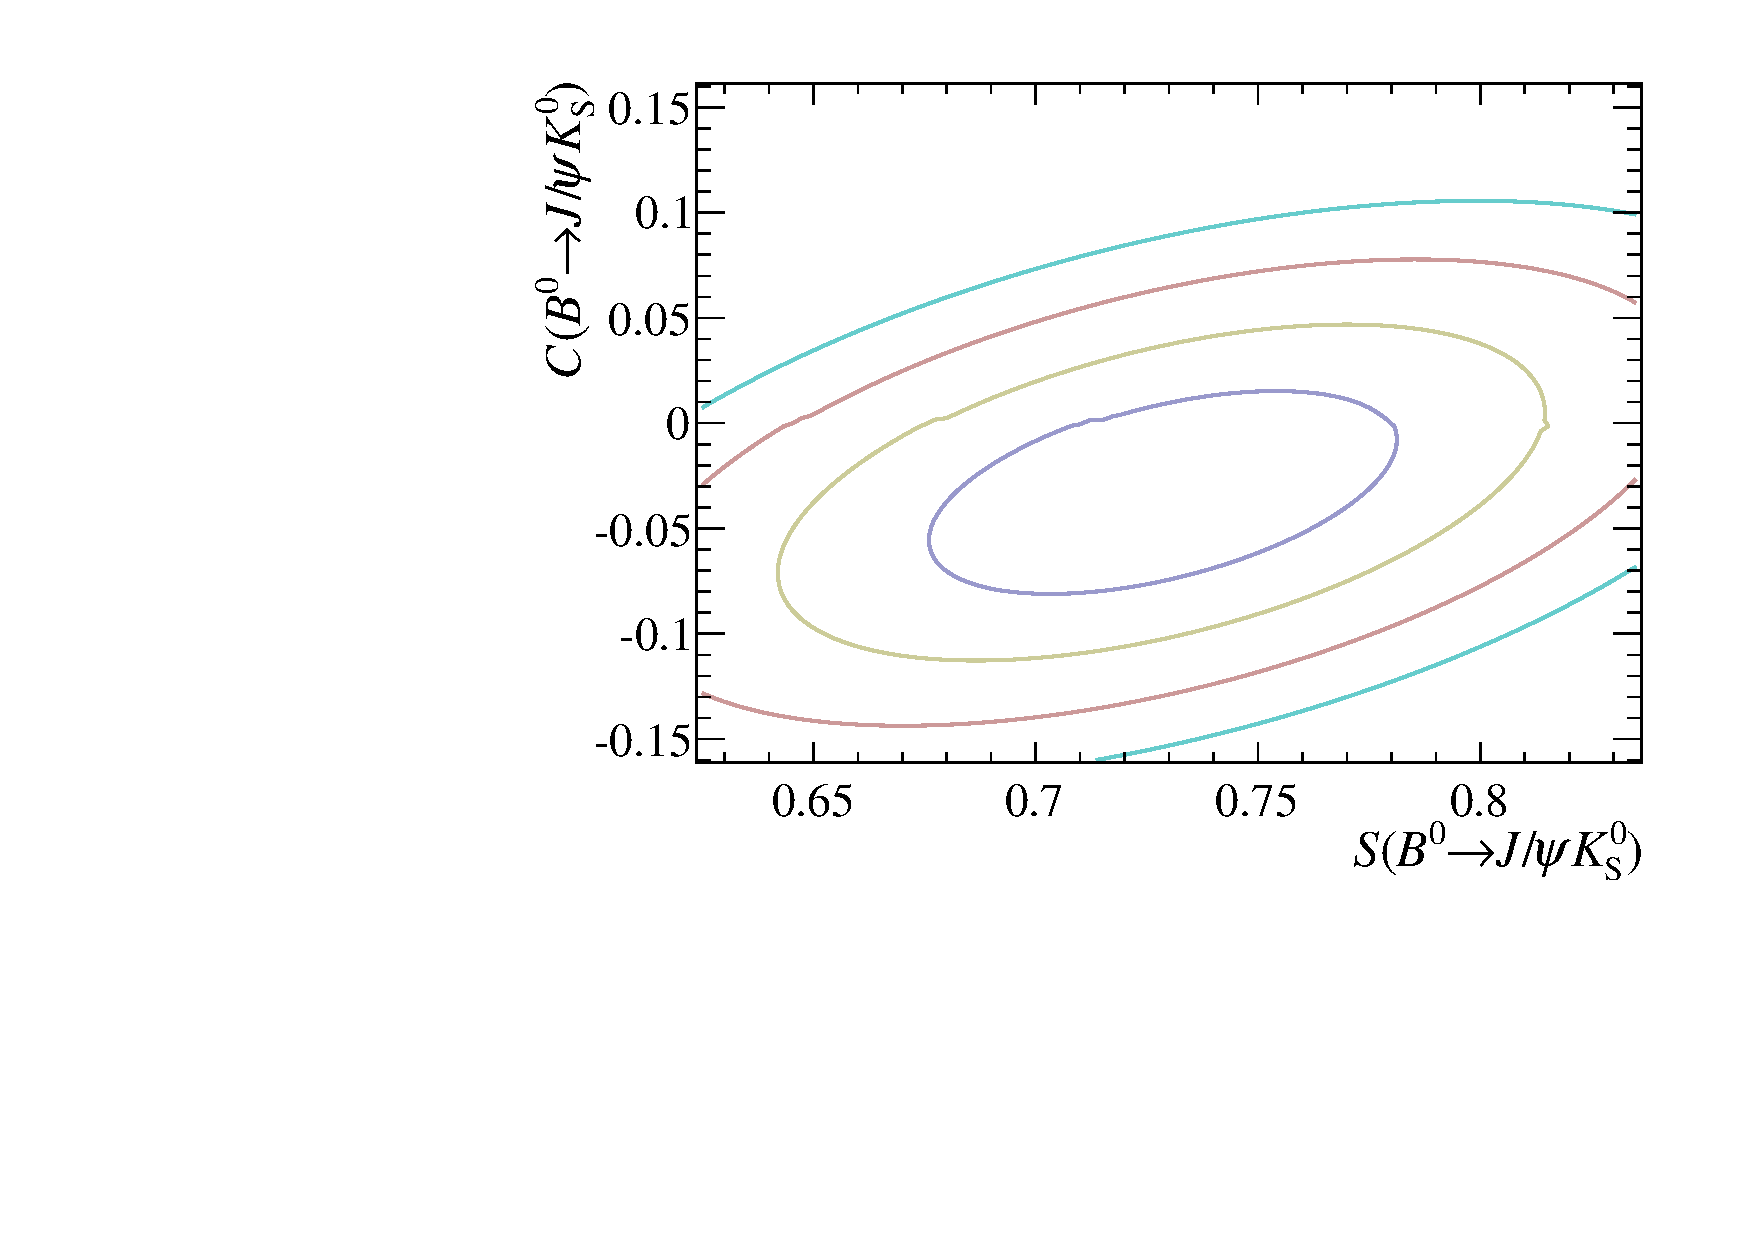
\includegraphics[width=1.00\textwidth]{private/content/measurement-of-sin2beta/figs/LLScan_2D.pdf} \\
  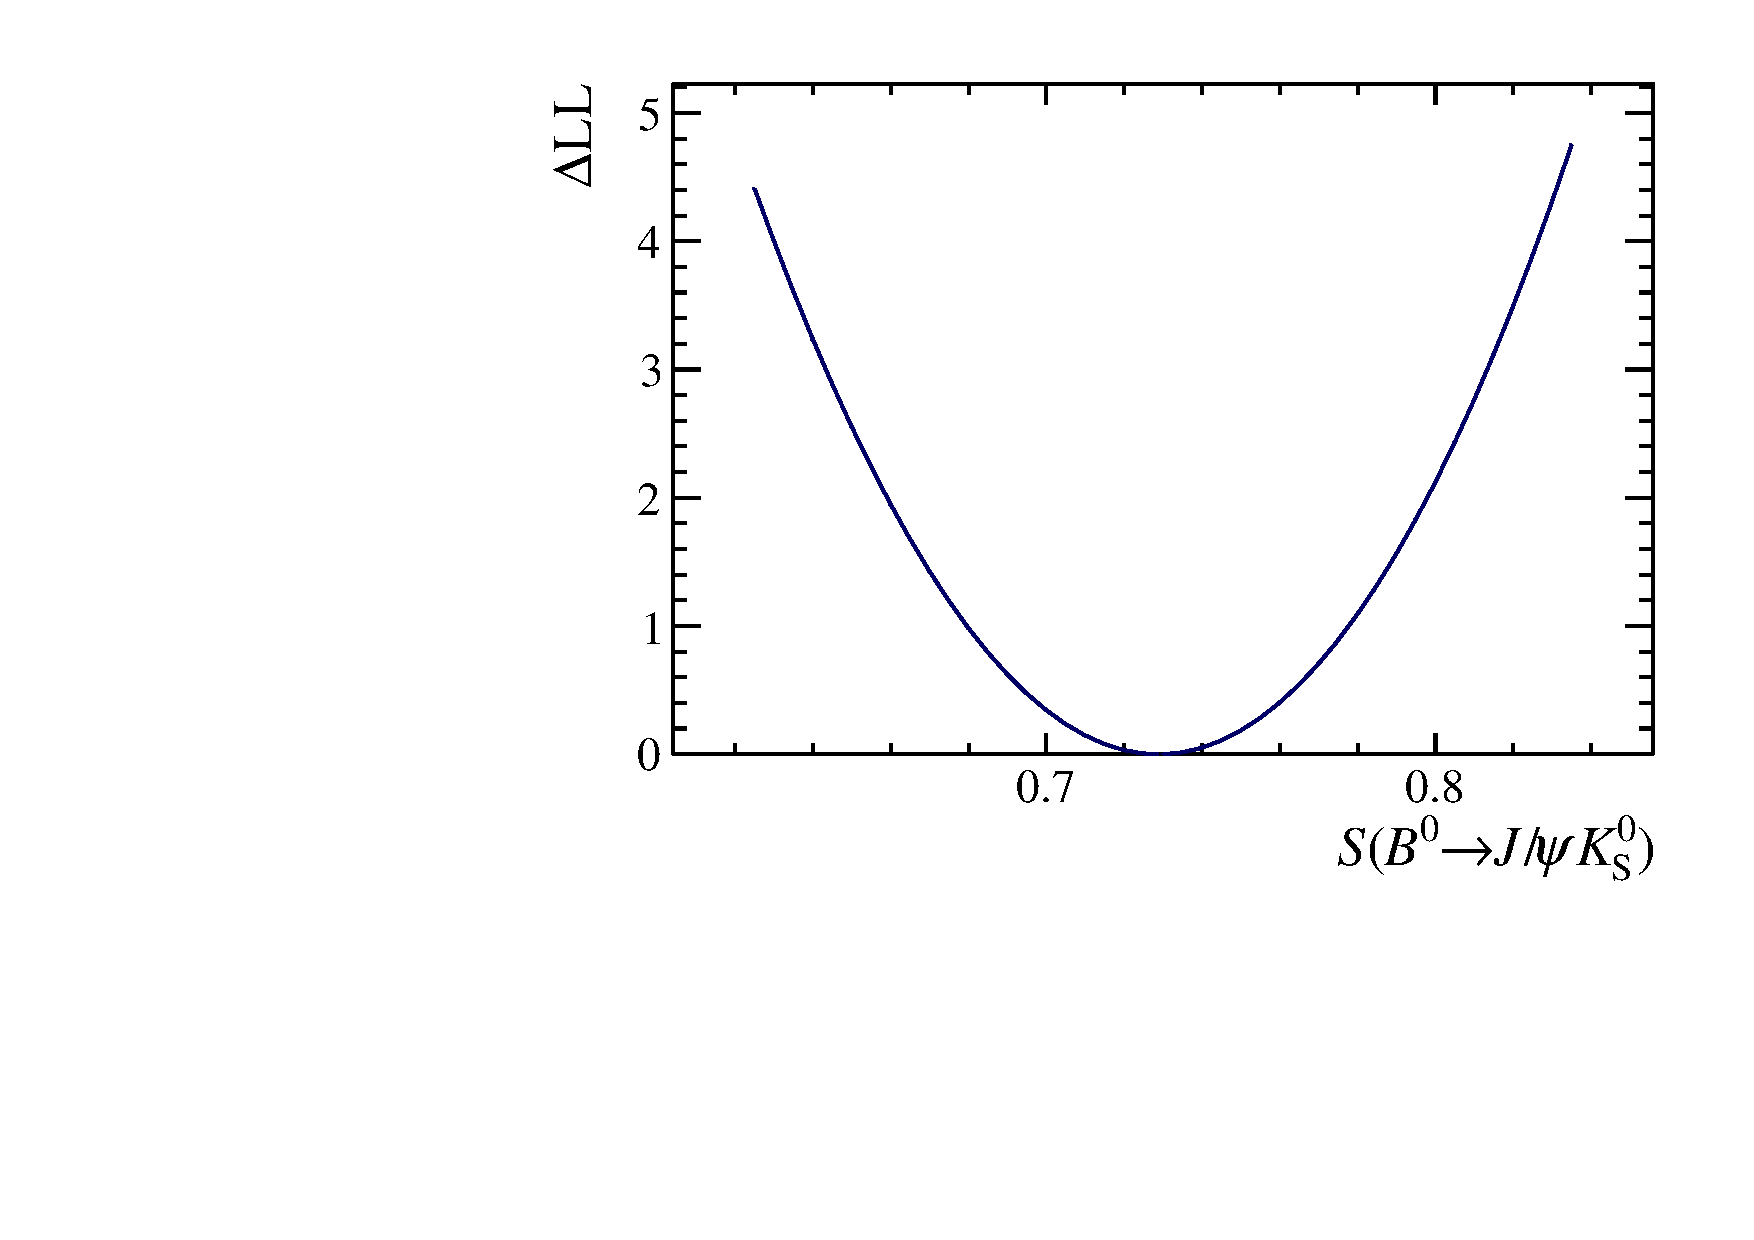
\includegraphics[width=0.46\textwidth]{private/content/measurement-of-sin2beta/figs/LLScan_1D_S.pdf}
  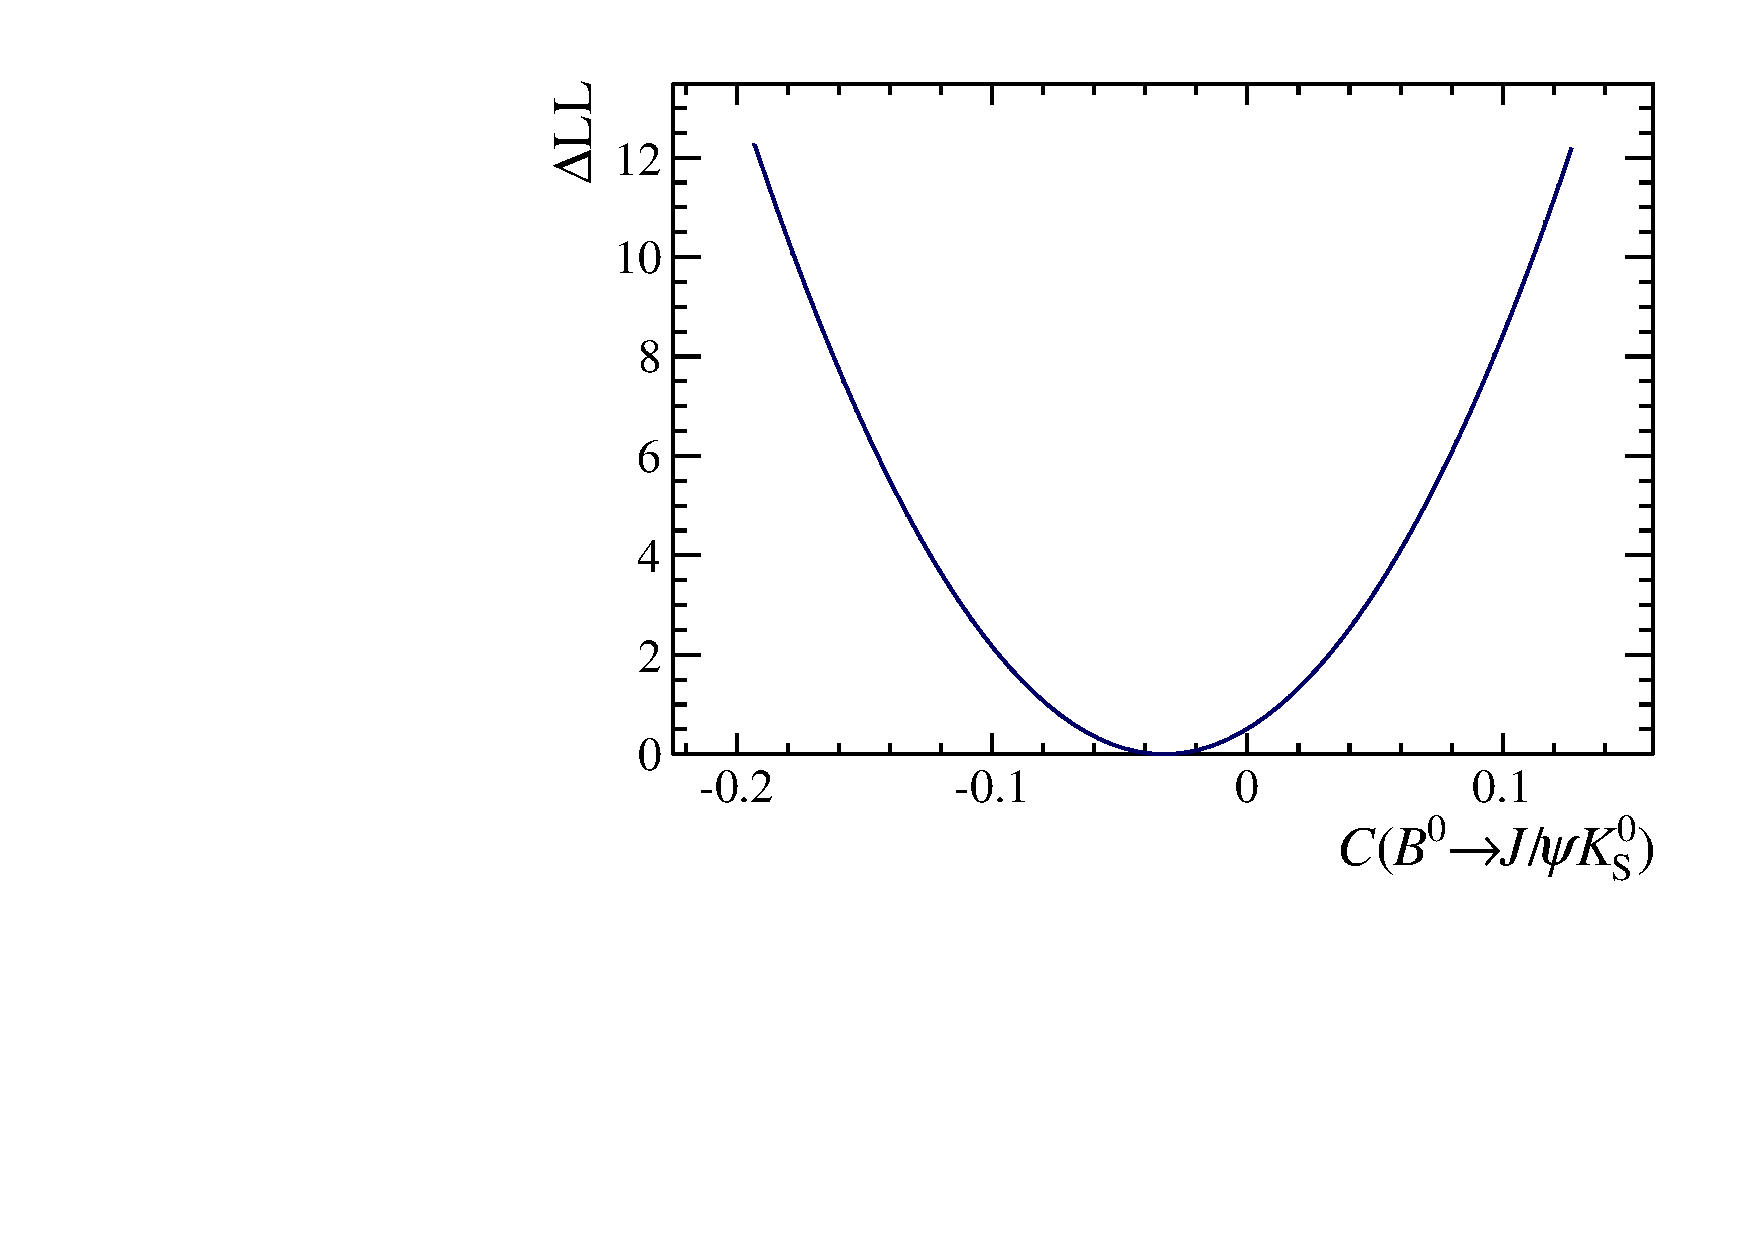
\includegraphics[width=0.46\textwidth]{private/content/measurement-of-sin2beta/figs/LLScan_1D_C.pdf}
  \caption{One and two dimensional likelihood profile scans for $\SJpsiKS$ and $\CJpsiKS$.}
  \label{fig:measurement_of_sin2beta:cpv_measurement:results:plots:ll_scan}
\end{figure}
